\title{linear equations in two variables}
%\usepackage{graphicx} % Required for inserting images

\documentclass[12pt]{article}
\usepackage{amsmath}
\newcommand{\myvec}[1]{\ensuremath{\begin{pmatrix}#1\end{pmatrix}}}
\newcommand{\mydet}[1]{\ensuremath{\begin{vmatrix}#1\end{vmatrix}}}
\newcommand{\solution}{\noindent \textbf{Solution: }}
\providecommand{\brak}[1]{\ensuremath{\left(#1\right)}}
%\providecommand{\norm}[1]{\left\lVert#1\right\rVert}
\let\vec\mathbf
\usepackage{graphicx}
\graphicspath{ {./images/} }

\title{Coordinate Geometry}
\author{harshita (paidisettyharshita@sriprakashschools.com)}

\begin{document}
\maketitle
\section*{Class 10$^{th}$ Maths - Chapter 7}
This is Problem-7 from Exercise 7.4
\begin{enumerate}
\item Find the coordinates of a point A, where AB is the diameter of a circle whose centre is (2, -3) and B is (1, 4).\\
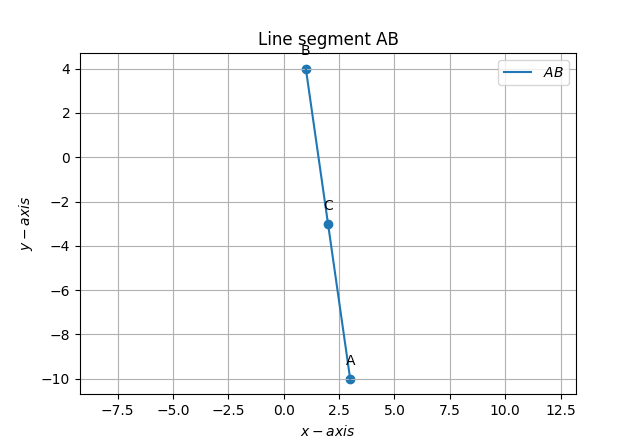
\includegraphics{/home/clab17/Figure_1.png}
\solution:
$c = \frac{x_1+x_2}{2} , \frac{y_1+y_2}{2}$\\
\begin{align}
c = (\frac{x+1}{2} , \frac{y+4}{2})\\
2 = \frac{x+1}{2} \\
x=3\\
so,\\
-3 =\frac{y+4}{2}\\
y=-10\\
\end{align}
hence,the coordinates are (3,-10)

\end{enumerate}
\end{document}